\documentclass{article}
\usepackage[margin=1in]{geometry}
\usepackage{amsmath,amsthm,amssymb}
\usepackage{bbm,enumerate,mathtools}
\usepackage{tikz,pgfplots}
\usepackage{chessboard}
\usepackage[hidelinks]{hyperref}
\usepackage{multicol} % Problem 35

\newenvironment{question}{\begin{trivlist}\item[\textbf{Question.}]}{\end{trivlist}}
\newenvironment{note}{\begin{trivlist}\item[\textbf{Note.}]}{\end{trivlist}}
\newenvironment{references}{\begin{trivlist}\item[\textbf{References.}]}{\end{trivlist}}
\newenvironment{related}{\begin{trivlist}\item[\textbf{Related.}]\end{trivlist}\begin{enumerate}}{\end{enumerate}}


\begin{document}
  Consider all of the ways to take a square piece of paper and make two
  ``precise'' creases---that is, we can make a crease between two distinguished
  points, we can crease the paper such that any two distinguished points touch,
  and we can take an angle and bisect it.
  \begin{figure}[ht!]
    \centering
    % Triangle
    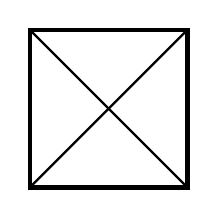
\begin{tikzpicture}
      \draw[ultra thick] (0,0) rectangle (2,2);
      \draw[thick] (0,0)--(2,2);
      \draw[thick] (2,0)--(0,2);
    \end{tikzpicture}
    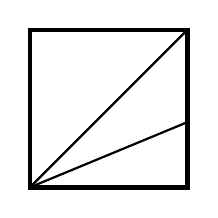
\begin{tikzpicture}
      \draw[ultra thick] (0,0) rectangle (2,2);
      \draw[thick] (0,0)--(2,2);
      \draw[thick] (0,0)--(2,0.828);
    \end{tikzpicture}
    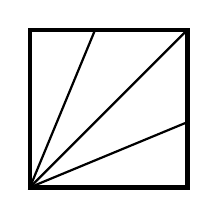
\begin{tikzpicture}
      \draw[ultra thick] (0,0) rectangle (2,2);
      \draw[thick] (0,0)--(2,2);
      \draw[thick] (0.828,2)--(0,0)--(2,0.828);
    \end{tikzpicture}
    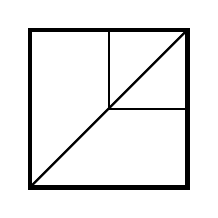
\begin{tikzpicture}
      \draw[ultra thick] (0,0) rectangle (2,2);
      \draw[thick] (0,0)--(2,2);
      \draw[thick] (1,2)--(1,1)--(2,1);
    \end{tikzpicture}
    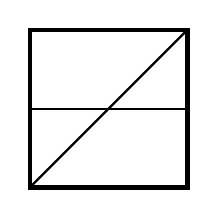
\begin{tikzpicture}
      \draw[ultra thick] (0,0) rectangle (2,2);
      \draw[thick] (0,0)--(2,2);
      \draw[thick] (0,1)--(2,1);
    \end{tikzpicture}
    % Horizontal
    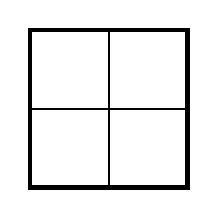
\begin{tikzpicture}
      \draw[ultra thick] (0,0) rectangle (2,2);
      \draw[thick] (0,1)--(2,1);
      \draw[thick] (1,0)--(1,2);
    \end{tikzpicture}
    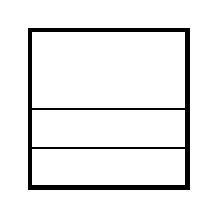
\begin{tikzpicture}
      \draw[ultra thick] (0,0) rectangle (2,2);
      \draw[thick] (0,1)--(2,1);
      \draw[thick] (0,0.5)--(2,0.5);
    \end{tikzpicture}
    \\\vspace{0.1cm}
    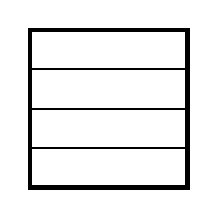
\begin{tikzpicture}
      \draw[ultra thick] (0,0) rectangle (2,2);
      \draw[thick] (0,1)--(2,1);
      \draw[thick] (0,0.5)--(2,0.5);
      \draw[thick] (0,1.5)--(2,1.5);
    \end{tikzpicture}
    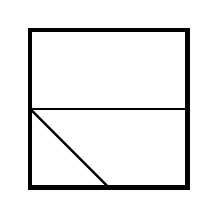
\begin{tikzpicture}
      \draw[ultra thick] (0,0) rectangle (2,2);
      \draw[thick] (0,1)--(2,1);
      \draw[thick] (0,1)--(1,0);
    \end{tikzpicture}
    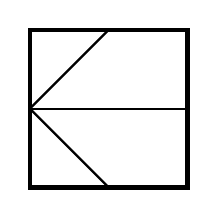
\begin{tikzpicture}
      \draw[ultra thick] (0,0) rectangle (2,2);
      \draw[thick] (0,1)--(2,1);
      \draw[thick] (1,2)--(0,1)--(1,0);
    \end{tikzpicture}
    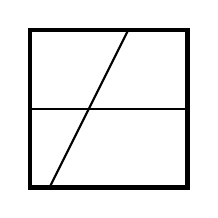
\begin{tikzpicture}
      \draw[ultra thick] (0,0) rectangle (2,2);
      \draw[thick] (0,1)--(2,1);
      \draw[thick] (0.25,0)--(1.25,2);
    \end{tikzpicture}
    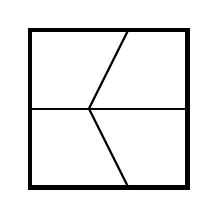
\begin{tikzpicture}
      \draw[ultra thick] (0,0) rectangle (2,2);
      \draw[thick] (0,1)--(2,1);
      \draw[thick] (1.25,0)--(0.75,1)--(1.25,2);
    \end{tikzpicture}
    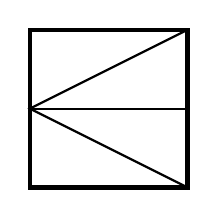
\begin{tikzpicture}
      \draw[ultra thick] (0,0) rectangle (2,2);
      \draw[thick] (0,1)--(2,1);
      \draw[thick] (2,0)--(0,1)--(2,2);
    \end{tikzpicture}
    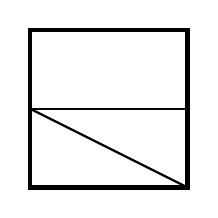
\begin{tikzpicture}
      \draw[ultra thick] (0,0) rectangle (2,2);
      \draw[thick] (0,1)--(2,1);
      \draw[thick] (2,0)--(0,1);
    \end{tikzpicture}
    \caption{
      Fourteen (all?) two-crease patterns.
    }
  \end{figure}
  \begin{question}
    How many such crease patterns exist on $n$ creases?
  \end{question}

  \begin{related}
    \item If we ``overlap'' all diagrams, how many distinct lines?
    \item What if we start with a rectangle? Equilateral triangle?
    \item What if $n$ is the number of folds, and unfolding counts as a fold?
    \item What if we restrict the possible folds---for example, disallow folding
    a crease between two distinguished points?
  \end{related}
  \begin{references}
    \item \url{https://en.wikipedia.org/wiki/Crease_pattern}
  \end{references}
\end{document}
